
\documentclass[11pt, a4paper]{article}

\usepackage[T1]{fontenc}
\usepackage{mathpazo}
\usepackage{graphicx}\graphicspath{{Images/}}
\usepackage[margin=1in]{geometry}
\usepackage{setspace}
\usepackage{caption,subcaption}
\usepackage[sort&compress, numbers]{natbib}
\usepackage{hyperref}
% \usepackage{algorithm}
% \usepackage{algpseudocode}
\usepackage[ruled,vlined,linesnumbered]{algorithm2e}
\usepackage{booktabs}
\usepackage{adjustbox}
\usepackage{graphicx}

\captionsetup{font={small, stretch=1}, labelfont=bf}
\renewcommand{\figurename}{Fig.}
\setlength{\bibsep}{3pt}
\newcommand{\Title}[1]{{\LARGE \centering \hrulefill\\ \textbf{#1}\\ \hrulefill}}
%==================================================================

\begin{document}

\pagenumbering{roman}
\pagestyle{plain}


\onehalfspacing
\setcounter{page}{1}
\pagenumbering{arabic}
\Title{Computational Experience with the Maximal Location Covering Problem}

\section*{Abstract}
{\small \singlespacing
	On this paper, you can find heuristic approaches applied to the Maximal Covering Location Problems; this project could be useful to decision makers that want to generate a solution and try to improve a given solution as well in a short amount of time.  
}

\section{Introduction}\label{sec:intro}
Facility Location is a branch of Operations Research. This category of combinatorial optimization problems often deals with problems that seek to select the placement of a facility (often, from a given list of possibilities) that meets the best of certain constraints. These problems often consists of minimizing the total weighted distances from supplies and customers, and weights are representative of the difficulty of transporting materials. 

Then, we have the Maximal Covering Location Problem. This problem is a derivative of Facility Location sort; however, this problems seeks to maximize the customers covered by a given set of facilities,instead of minimizing the distance between customers and supplies. 

The Maximal Covering Location Problem (MCLP), is a classic problem in location analysis with    applications in a good number of fields, such as health care, emergency planning, ecology, statistical classification, homeland security, etc.

The objective of the MCLP is to maximize the population covered by a given set of facilities; however, this could work as an analogy to another problems that involve "supply" and "demand" points to maximize the demand as much as possible.

Formally, this problem is described in Church and ReVelle 1974 as follows:
"The maximal covering location problem seeks the maximum population which can be served within a stated service distance or time given a limited number of facilities."

In this work, MCLP is analysed and solved on random instances generated within a certain range, by an implemented instance generator. A Constructive Heuristic approach was used to generate a solution, and a Local Search algorithm was implemented to try to improve the feasible solution generated by the constructive. Overall, the effectiveness and computational time of the implemented algorithms on small, medium and large instances were analysed. More details are given in the following sections.

\section{Problem description - Mathematical model}\label{sec:lit}
According to the model defined on Church and ReVelle 1974, this problem is defined on a network of nodes and arcs. 

A mathematical formulation of this problem can be stated as Eq. ~\ref{eq: math model}:

\begin{equation}\label{eq: math model}
	max \; z = \sum_{i \in I}y_i
\end{equation}
subject to:

\begin{equation}\label{eq: r1}
	x_{j} \in (0,1), j \in J
\end{equation}

\begin{equation}\label{eq: r2}
	y_{i} \in (0,1), i \in I
\end{equation}

\begin{equation}\label{eq: r3}
	\sum_{j \in J}x_j = S
\end{equation}

\begin{equation}\label{eq: r4}
	\sum_{j \in N_i} x_j \geq y_i, N_i = \big\{ j \in J: d_{ij} \leq r \big\}
\end{equation}
where

\begin{itemize}
	\item $x_{j}$ : denotes that the $j$-th facility site is selected (1) or not (0). Boolean variable.
	\item $y_{i}$ : denotes that if the demand point i is covered by any facility site within radius $r$ (1) or not (0). Boolean variable.
	\item $I$ : the set of demand or population points. Array of indexes referencing the coordinates of each demand point.
	\item $J$ : the set of facility candidate sites. Array of indexes referencing the supply points.
	\item $d(i,j)$ : the Euclidean distance from a demand point $i$ to facility site $j$. 2-D matrix.
	\item $S$ : the number of desired facilities to be selected from the candidate sites $J$. Integer variable.
	\item $r$ : Maximal distance where a demand point from set $I$ is covered by a facility site from set $J$. Integer variable.
\end{itemize}
The objective is to maximize the number of demand points covered within a desired service distance, as depicted in ~\ref{eq: math model}.
A selection criteria for a site is described in restriction ~\ref{eq: r1}, where as restriction ~\ref{eq: r2} alludes to all the demands point covered within a specified radius. Ideally, the sum of the selected sites must be equal to the desired by a decision maker as stated on restriction ~\ref{eq: r3}; however, it's possible that all the demand/population points are covered before this restriction is satisfied. Restriction ~\ref{eq: r4} indicates that the distance between covered nodes by the selected sites must be under the specified radius from the user.

\subsection{Example}
The scatter plot shown in the figure ~\ref{fig:example_instance_input} was generated by an instance generator coded in the programming language Python. The range of the population points are within a range of 5-500 units, and the potential candidate sites were generated inside the convex hull of the demand points. There are exactly 500 demand points, and 20 candidate sites. The values were generated randomly.

\begin{figure}[h]
	\centering
	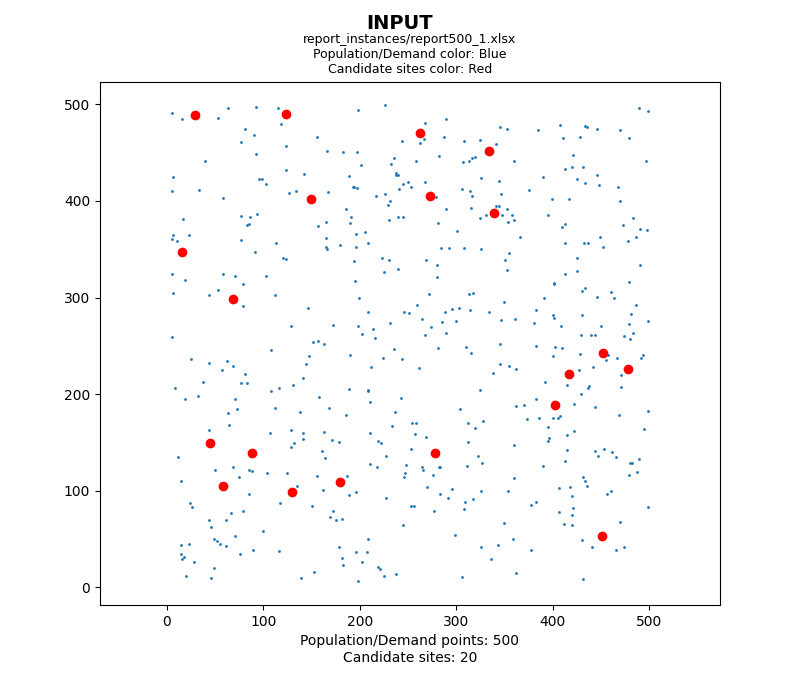
\includegraphics[scale=0.8]{example_instance_input.png}
	\caption{Random instance of population and candidate sites points}
	\label{fig:example_instance_input}
\end{figure}

As shown, the population points are illustrated in the scatter plot in blue, and the potential candidate sites are filled with red.

Once the input is succesfully computed, there are a few ways to figure out a first feasible solution. As seen in Church and ReVelle 1974, a first heuristic approach called Greedy Adding (GA) was considered. This approach starts with an empty solution, and starts to iterate each candidate site until the one with maximal covered population is found; then, this site is added to the solution. It keeps iterating until either the $S$ facilities have been selected or all the population is covered. However, there is a problem with this approach: the time complexity is denoted as $O(n \ logn)$, which means that it's not efficient for big instances.

Instead of using the Greedy Adding algorithm proposed by these guys, a Constructive Heuristic approach was implemented for generating first a feasible solution that meet the constraints. Then, a Local Search move approach tries to improve this solution. These heuristics are discused in more detail on the following sections.

\begin{figure}[h]
	\centering
	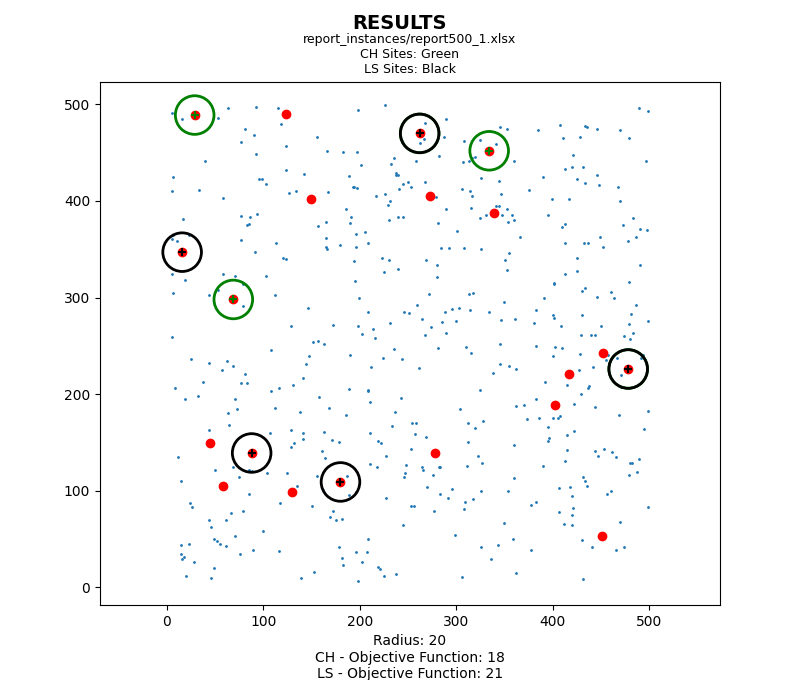
\includegraphics[scale=0.8]{example_instance_output.png}
	\caption{Random instance of population and candidate sites points}
	\label{fig:example_instance_output}
\end{figure}

The scatter plot shown in the figure ~\ref{fig:example_instance_output} illustrates the output of the applied heuristics mentioned previously. The sites and population covered of the Constructive Heuristic approach are marked with green circles, and black circles illustrate the ones covered by Local Search. 

\section{Heuristics}\label{sec:exp}

\subsection{Description of Constructive Heuristic}
By definition, a constructive heuristic is a type of heuristic that starts with an empty solution and keeps extending with each iteration until a feasible solution is obtained.

The implementation of the Constructive Heuristic made for this problem receives as input the demand points $I$, the potential candidate sites $J$, the desired sites to be selected $S$ and the $radius$ of coverage.
The Constructive Heuristic implemented for the MCLP is described in the Alg. ~\ref{pseudo: ch}.

\begin{algorithm}[H]
	\caption{Constructive Heuristic}\label{pseudo: ch}
	\SetAlgoLined
	\SetKwInput{KwInput}{Input}
	\SetKwInput{KwOutput}{Output}
	\SetKwInput{KwResult}{Pseudocode}
	\SetKw{KwBy}{in}
	\DontPrintSemicolon

	\KwInput{\begin{itemize}
		\item $I \gets [1,2,3...i]$\;
		\item $J \gets [1,2,3...j]$
		\item $S \gets int \ value$
		\item $radius \gets int \ value$
	\end{itemize}}
	\KwOutput{\begin{itemize}
		\item $selected\_sites \gets [1,2,3...S]$
		\item $objective\_function \gets Population \ covered \ by \ selected\_sites$
	\end{itemize}}
	\KwResult{}
	$selected\_sites \gets []$\;
	$population\_size \gets length(I)$\;
	\BlankLine
	\BlankLine
	\For{$site$ \KwBy $J$}{
		$current\_covered\_nodes \gets Compute \ covered \ nodes (selected\_sites)$\;
		$objective\_function = length(current\_covered\_nodes)
		$\;
		\BlankLine
		$r1 = covered\_nodes(under \ radius(site)) > 0$\;
		$r2 = length(selected\_sites) < S$\;
		$r3 = objective\_function < population\_size$\;
		\BlankLine
		\uIf{(r1 and r2 and r3) == True}{
			$Append \ site \ to \ selected\_sites$\;
		}\uElseIf{r1 == False}{
			$pass$\;
		}\uElse{
			$return \ selected\_sites,\ objective\_function$\;
			$break \ for$\;
		}
	}
	
\end{algorithm}

\subsection{Description of Local Search}
Before describing the move of the Local Search (LS) algorithm used on this problem, it's important to know what a Local Search is; the main thing that differs between Local Search and Constructive heuristics is that Local Search needs a starting solution, whereas Constructive heursitics starts with a empty solution and build it from scratch. 

In general, the objective of Local Search moves is to improve a given solution. Best-found strategy was used in the LS implementation for the MCLP, described in the alg. ~\ref{pseudo: ls}.
\paragraph{$Move(j,k):$}
Replace open facility $j$ (currently in objF\_sites[]) by a free candidate site $k$ (currently in free\_sites[]) 

\begin{algorithm}
	\caption{Local Search heuristic}\label{pseudo: ls}
	\SetAlgoLined
	\SetKwInput{KwInput}{Input}
	\SetKwInput{KwOutput}{Output}
	\SetKwInput{KwResult}{Pseudocode}
	\SetKw{KwBy}{in}
	\DontPrintSemicolon

	\KwInput{\begin{itemize}
		\item $objF\_value \gets current \ objective \ function$
		\item $objF\_sites \gets [1,2,3...S]$
		\item $free\_sites \gets [1,2,3...j] \ from \ J \ not \ in S$
		\item $sites\_with\_obj\_F \gets $ \big\{j in J: obj\_F of j\} dict
	\end{itemize}}
	\KwOutput{\begin{itemize}
		\item $new\_sites\_set \gets [1,2,3...new(S)]$
		\item $new\_objF \gets Population \ covered \ by \ new\_sites\_set$
	\end{itemize}}
	\KwResult{}
	$objF\_copy \gets copy(objF\_value)$\;
	$objF\_sites\_copy \gets copy(objF\_sites)$\;
	$free\_sites\_copy \gets copy(free\_sites)$\;
	$sites\_with\_objF\_copy \gets copy(sites\_with\_objF)$\;
	\BlankLine
	\BlankLine
	\For{$site$ \KwBy $objF\_sites\_copy$}{
		$site\_objF \gets sites\_with\_objF\_copy[site]$\;
		\BlankLine
		
		\For{$free\_site$ \KwBy $free\_sites\_copy$}{
			$free\_site\_objF = sites\_with\_objF\_copy[free\_site]$\;
			\BlankLine
			\uIf{free\_site\_objF > site\_objF}{
				$objF\_sites\_copy[site] \gets free\_site$\;
			}
			\uElse{
			$pass$\;
			}
		}
	}
	\BlankLine
	\BlankLine
	$new\_sites\_set \gets objF\_sites\_copy$\;
	$new\_objF \gets Population \ covered \ by \ new\_sites\_set$\;
	\BlankLine
	\uIf{free\_site\_objF > site\_objF}{
		$return \ new\_sites\_set, new\_objF$\;
	}
	\uElse{
		$print \ "Solution \ couldn't \ be \ improved"$\;
	}
\end{algorithm}

\section{Experiments}
Experiments and testing of implementations of Constructive and Local Search heuristics seen in alg. ~\ref{pseudo: ch} and alg. ~\ref{pseudo: ls} were coded on Python programming language, and they were tested on a computer with an Intel Core i7-6500u processor. Basic frequency of this processor is between 2.5-3.1 GHz.

\begin{table}[h!]
\centering
\begin{adjustbox}{max width=\textwidth}
% Pandas dataframe start
\begin{tabular}{lrrrrrl}
	\toprule
			 INSTANCE &  CH\_OF &  CH\_time (cpu sec) &  LSH\_OF &  LS\_time (cpu sec) &  ABSOLUTE IMP & RELATIVE IMP \\
	\midrule
	  small500\_1.xlsx &     54 &           0.349726 &      63 &           0.000037 &             9 &       16.67\% \\
	  small500\_2.xlsx &     73 &           0.036091 &      76 &           0.000232 &             3 &        4.11\% \\
	  small500\_3.xlsx &     65 &           0.033529 &      69 &           0.000201 &             4 &        6.15\% \\
	  small500\_4.xlsx &     61 &           0.032695 &      62 &           0.000249 &             1 &        1.64\% \\
	  small500\_5.xlsx &     54 &           0.032827 &      63 &           0.000157 &             9 &       16.67\% \\
	  small500\_6.xlsx &     68 &           0.014754 &      76 &           0.000169 &             8 &       11.76\% \\
	  small500\_7.xlsx &     66 &           0.013740 &      73 &           0.000156 &             7 &       10.61\% \\
	  small500\_8.xlsx &     64 &           0.013012 &      68 &           0.000172 &             4 &        6.25\% \\
	  small500\_9.xlsx &     51 &           0.032844 &      71 &           0.000202 &            20 &       39.22\% \\
	 small500\_10.xlsx &     54 &           0.015027 &      61 &           0.000120 &             7 &       12.96\% \\
	 small500\_11.xlsx &     55 &           0.033229 &      59 &           0.000101 &             4 &        7.27\% \\
	 small500\_12.xlsx &     47 &           0.016532 &      58 &           0.000529 &            11 &       23.40\% \\
	 small500\_13.xlsx &     59 &           0.034043 &      74 &           0.000201 &            15 &       25.42\% \\
	 small500\_14.xlsx &     49 &           0.033183 &      76 &           0.000244 &            27 &       55.10\% \\
	 small500\_15.xlsx &     58 &           0.014746 &      78 &           0.000183 &            20 &       34.48\% \\
	 small500\_16.xlsx &     44 &           0.015279 &      70 &           0.000199 &            26 &       59.09\% \\
	 small500\_17.xlsx &     62 &           0.014306 &      71 &           0.000162 &             9 &       14.52\% \\
	 small500\_18.xlsx &     49 &           0.013388 &      70 &           0.000186 &            21 &       42.86\% \\
	 small500\_19.xlsx &     64 &           0.014963 &      66 &           0.000165 &             2 &        3.12\% \\
	 small500\_20.xlsx &     72 &           0.014259 &      72 &           0.000110 &             0 &        0.00\% \\
	\bottomrule
	\end{tabular}	
% Pandas dtaframe end

\end{adjustbox}
\caption{Small instances - Demand: 500[5-500], Candidate sites: 10, Selected sites: 4, Radius: 50}
\label{tab:small_instances}
\end{table}
\centering
Average improvement of instances of table ~\ref{tab:small_instances} = 19.57\%

\section{Conclusions}
Conclusions show readers the value of your completely developed argument or thoroughly answered question. Consider the conclusion from the reader's perspective. At the end of a paper, a reader wants to know how to benefit from the work you accomplished in your paper. 

\appendix
\section{Supporting information}
The purpose of the supporting information is to enable authors to provide and archive supporting information such as data tables, method information, figures, video, or computer software, in digital formats so that other scientists can use it.

\small \singlespacing
\bibliographystyle{unsrtnat} 
\bibliography{mybib}

\end{document}









 





















